\documentclass[unicode,11pt,a4paper,oneside,numbers=endperiod,openany]{scrartcl}

 \setlength{\abovecaptionskip}{-10pt}

\input{assignment.sty}
\begin{document}


\setassignment
\setduedate{13.10.2020 (midnight)}

\serieheader{High-Performance Computing Lab}{2020}{Student: Gabriele Berra}{Discussed with: -}{Solution for Project 1}{}
\newline

\assignmentpolicy
In this first assignment I will tackle - fist theoretically and then practically - one of the most important aspect to take in consideration when coding in order to reach the highest performance out of our machines: the memory hierarchies. 

\section{Explaining Memory Hierarchies \punkte{30}}
\subsection{Introduction}
In order to understand the memory hierarchies we first have to consider which types of memory exist and the relationship between each one. Basically, we can distinguish memories for their speed in accessing the data (i.e. the time - usually in nanoseconds - between the request of the data and when the data is received) and for their capacity of storing a large amount of them. Starting from the farthest from the Arithmetic Unit (AU) - which is the unit that receives data from the register and performs operations on them - we find the main memory, the biggest and also the slowest, capable of storing large amount of data. The second memories are the cashes which are smaller than the main memory but are fastest since they are closer to the AU. Starting from the biggest - and also the closest (physically) to the main memory - we find: Level 3 cache (L3), Level 2 cache (L2), Level 1 cache (L1). Last but not least, a fundamental memory very close to the AU - and, for this reason, the fastest - is represented by the registers.

Once we have understood the differences between the various types of memories, both on the basis of their size and their speed in accessing the data, we will focus on the relationship between them. As said before, the AU is the unit that sends the request for a specific data. The latter is searched, firstly, in the registers and, if it is not present there, the AU searches for it in the L1 cache, then in L2 and so on. Finally, the last memory in which the AU has to search is the main memory. Now, it is easy to understand that, in order to reach high performance, it is necessary to load the data that we are going to use in the closest memory, so that the AU spends less time searching for it, thus improving the performance. Once understood what the different memories are and how they work, we can focus our attention on how to use them efficiently considering their different capacity. The perfect - and also utopistic - situation is when all the data that we are going to use in our computation are in the L1 cache. Unfortunately for us, we can load only few data in L1, but if we can manage to use as much as possible the data loaded in it, then the AU does not have to search in other memories and, thus, the computational speed increases. Every time that the data that we search is present in the caches is called a \textit{cache hit}. In contrast, if the data that we need is not in the caches, that is called a \textit{cache miss} and, then, the AU has to load it directly from main memory, compromising the performance.

At the end of this introduction we can state that, if we want to reach the higher performance possible, we have to minimize the \textit{cache misses} during the process, by using as much as possible the data already loaded in the caches. We could also consider the time of the AU in performing the computations but, since that time cannot be modified, we focus our attention only on minimizing the \textit{cache misses} or, conversely, on maximizing the \textit{cache hits}.

\subsection{Identify the parameters of the memory hierarchy on the compute node of the ICS cluster}
The ICS cluster is a collection of computers called \textit{nodes} with different characteristics. In the ICS cluster there are 32 nodes CPU only, 8 with only one GPU, and 2 multi GPU. 

With the aim of obtaining the specifics of a node we have to:
\begin{itemize}
	\item Run the command \textit{likwid-topology} that gives as output the sizes of each cache and,
	\item run the command \textit{cat /proc/meminfo} that gives more information regarding the main memory, the memory available, and other useful parameters.
\end{itemize}
In my case, I took into consideration two nodes to better understand the differences. In the specific, those nodes are the \textit{login node} and \textit{node07}. I considered the latter since, as we can see with the command \textit{sinfo}, it has a big memory and, for this reason, I think it is appropriate to include it in my report regarding the memory hierarchies.

To be more precise, and also to answer the first question, I include below two tables containing both the sizes of the caches and of the main memory in the cases - respectively - of the \textit{login node} and of \textit{node07}.

\vspace{0.5cm}
\parbox{.45\linewidth}{
\centering
\begin{tabular}{|c|c|}
	\hline
	\multicolumn{2}{|c|}{ICS login node} \\
	\hline
	Main memory & 62.5443 GB \\
	\hline
	L3 cache &25 MB \\
	\hline
	L2 cache &256 kB \\
	\hline
	L1 cache &32 kB \\
	\hline
\end{tabular}
}
\hfill
\parbox{.45\linewidth}{
\centering
\begin{tabular}{|c|c|}
	\hline
	\multicolumn{2}{|c|}{ICS node07} \\
	\hline
	Main memory & 503.5439 GB \\
	\hline
	L3 cache &25 MB \\
	\hline
	L2 cache &256 kB \\
	\hline
	L1 cache &32 kB \\
	\hline
\end{tabular}
}
\vspace{0.5cm}

Since the data gathered from the cluster regarding main memory are in kB, for the computation of the size of it in GB I used the formula 1 GB = 1024 MB and 1 MB = 1024 kB. 

At a first glimpse at the tables, we can notice that the two nodes differs only in the size of the main memory, while the amount of data that can be stored in the caches is the same for each node taken in consideration. In conclusion, if we have to deal with an enormous amount of date we are going to use the ICS node07 instead of any other node.\footnote{I will, however, never run anything on the login node, since I do not want strict actions to be taken against me. =(}

\subsection{Running \textit{membench} on the ICS cluster and on my local machine}
The two figures below were given by running the \textit{run\_membench.sh} file: figure \ref{fig:membenchlocal} refers to the results obtained on my local machine, while figure \ref{fig:membenchcluster} refers to the results obtained on the cluster.

\begin{figure}[h!]
	\centering
	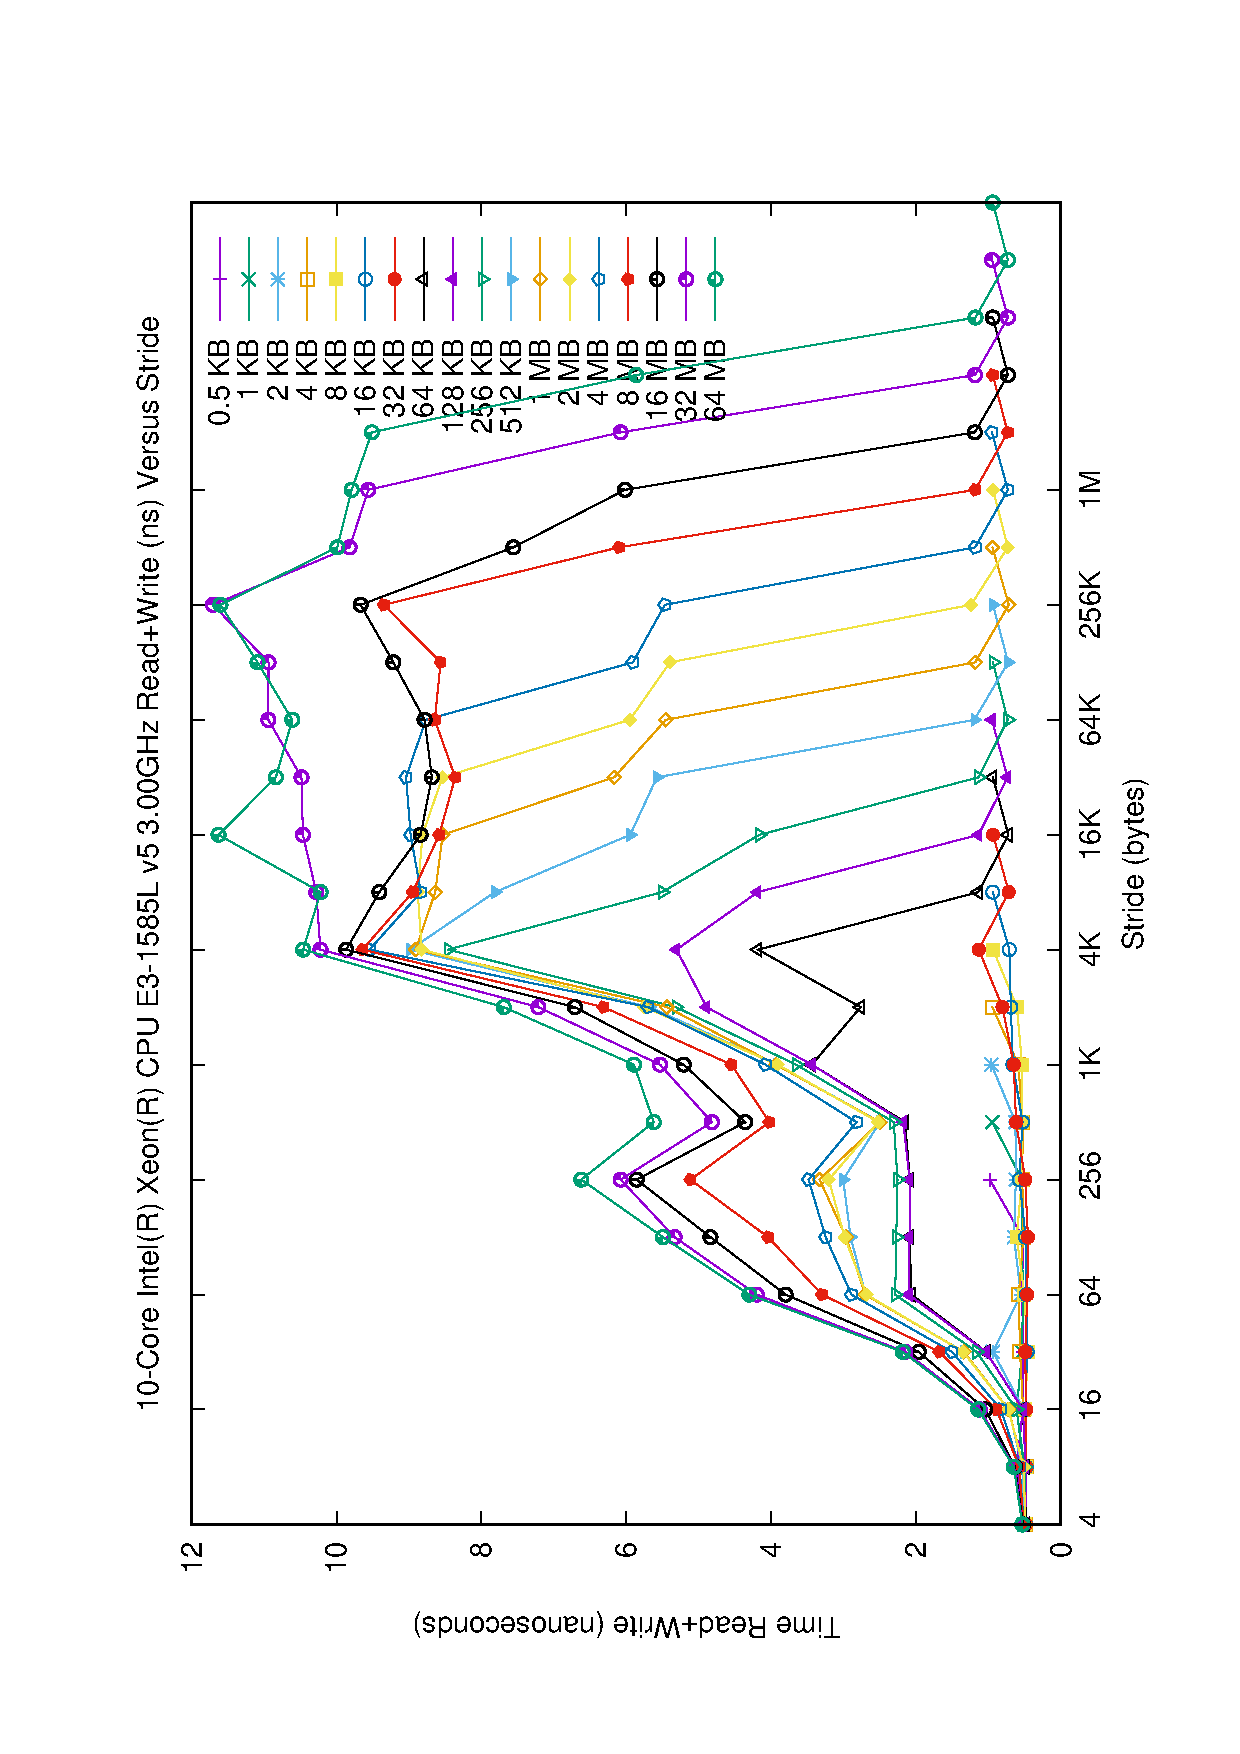
\includegraphics[width=0.82\textwidth]{Figures/local_results.pdf}
	\caption{Results of \textit{run\_membench.sh} on a mid 2014 Macbook Pro with 2.2 GHz Intel Core i7.}\label{fig:membenchlocal}
\end{figure}
\begin{figure}[h!]
	\centering
	\includegraphics[width=0.90\textwidth]{Figures/generic.pdf}
	\caption{Results of \textit{run\_membench.sh} on the USI ICS cluster.}\label{fig:membenchcluster}
\end{figure}

\subsection{Memory access pattern in specific cases}
We can now consider the memory access pattern in the specific cases reported below. Please notice that the same behaviour applies both to my local machine and to the ICS cluster.
\begin{itemize}
	\item \textit{csize = 128} and \textit{stride = 1} \\ In this case we are looking at the first point in the x-axis in which all the values in the cache are very close one to another and, thus, the ratio between the cache hit and cache miss is high (more cache hit than cache miss). In this case we can benefit from spatial locality due to the relative proximity in memory of the data point we are trying to fetch.
	\item \textit{csize} $= 2^{20}$ and \textit{stride} $ = csize/2$ \\ In this second case we are looking at the array of 8MB with a stride of 4MB. This means that we are accessing only two memory locations that can be contained in L1. In fact, as we can see from the graph, the ending point of the 8MB array is - talking in nanoseconds - in the lower part of the figure and we know from the theory that in that part the data needed for the computation can be easily stored in the L1 cache. Furthermore, in this case we can somehow benefit from temporal locality, since the memory benchmark test is repeated multiple times (see the next section on this).
\end{itemize}

\subsection{Analysis of the output of \emph{generic.ps}}

My local machine is a mid 2014 Macbook Pro with 2.2 GHz Intel Core i7. The size of the L1, L2 and L3 caches is the same as the ones on the cluster, while the clock speed is lower (indeed, by running \emph{cat /proc/cpuinfo}, I obtained that the cluster has roughly 2601 MHz).

From the observation of figure \ref{fig:membenchlocal} and figure \ref{fig:membenchcluster} we can notice that, in general, arrays with small stride allow better to exploit spatial locality. This is due to the fact that, when we load into the caches a chunk of data from main memory, we are going to have less cache misses than expected, since the data we are accessing are relatively contiguous in memory. However, we can notice also that the memory benchmark test is repeated many times, so we benefit also from temporal locality. This last point is particularly evident in the last part of every line, where the value of the stride approaches half of the length of the test vector. In these cases, we have a few values that can be stored in L1 or L2 caches and, when they are accessed multiple times in a row to perform the test, this leads to the good results which can be observed in the plot (access time of below 2 nanoseconds in the case of the cluster, and below 5 nanoseconds in the case of my local machine).

From the figures we can also observe some jumps connected to the increase of the size of the test array. These jumps are caused by the fact that the array is bigger than a given level of cache and, for this reason, the data has to be stored in the next cache level. If we take into account figure \ref{fig:membenchcluster}, we can observe a first jump in correspondence of an array size of 64kB: this is due to the fact that the L1 cache size is only 32kb, and the data considered does not fit into it anymore (and, thus, the data has to be stored into the L2 cache). A second jump can be noticed in correspondence of an array size of 512kb, when L2 is full and we are forced to store our data into L3. Finally, in the right part of the plot, with an array size of 32MB and 64MB a relatively high stride value (i.e., when we are not accessing anymore relatively contiguous locations in memory), we cannot store anymore our data into the L3 cache and we are forced to fetch them directly from main memory, thus obtaining bad timings of around 25 nanoseconds.

A similar general behaviour as the one explained above for the ICS cluster can be found also on my local machine, as observed in figure \ref{fig:membenchlocal}. In this case, the overall access time are generally worse, probably due to the lower clock rate with respect to the cluster. In particular, in the case of my local machine, we can notice that the stride value has a higher negative impact on the access time when comparing the results with the ones obtained on the cluster.


\section{Optimize Square Matrix-Matrix Multiplication  \punkte{70}}
In this second section I am going to describe the steps that lead me to the implementations of the \textit{blocked matrix multiplication} and to compare the performance achieved both on the ICS cluster and on my local machine (more details on the specific architecture can be found in the dedicated section). After having analyzed the problem, I decided to tackle it in two parts:
\begin{enumerate}
	\item Implementation of the blocked matrix multiplication by taking in consideration only matrix sizes that are multiples of the block size;
	\item Extension of my code in order to compute the blocked matrix multiplication for any block size and matrix size (thus handling also irregular matrix sizes like, e.g., prime numbers).
\end{enumerate}
 

\subsection{Step 1: From naive to blocked with block size multiple of the matrix size}
In this first part of the implementation I had to tackle two different problems:
\begin{enumerate}
	\item Understanding the best way to index the matrices in order to exploit the concepts of spatial locality and temporal locality.
	\item Introducing three additional loops and a new set of indices, in order to access the different blocks and perform matrix-multiplication in a more efficient way.
\end{enumerate}
As far as concerns the first problem, I had some troubles, initially, in understanding how the data was accessed in the naive matrix multiplication. Indeed, we are, actually, giving as input to the functions vector in column-major order and this implied the multiplication of the columns of $A$ and of the rows of $B$ in order to achieve the same results as in $AB=C$. The three for loops of the naive matrix multiplication are used for moving between the rows (i), the columns (j) and inside the matrix (k). I decided to keep the same structure in my blocked matrix implementation as well, since this appeared to me as the most efficient way to exploit the spatial and temporal locality discussed during the class (provided that the block size chosen is adequate with respect to the dimension of the cache of the machine).

After understanding how the loops were accessing the data in the matrix and how the output was stored in matrix $C$ (also in column-major format), I developed a small Matlab prototype that I used to debug the results obtained with my C implementation, along with a \emph{test.c} script that I used to perform the multiplication between two known matrices, in order to check the correctness of my results. In \emph{test.c} I implemented also a short function to print the result of the matrix multiplication on screen, so that I could compare with the results obtained with the Matlab prototype. After setting up my "debugging environment", I was ready to tackle the second problem, i.e. implementing three more loops in order to do the matrix multiplication block by block.  

At the beginning, I had some troubles with the implementation, mainly because I am new to C and I was unsure on how to exactly handling the indices. After fixing a bug related to $kb$ (i.e., the index governing the way in which we move along a given column or row of boxes), I was finally able to obtain the correct results. I have to stress that, however, in this first part I modified the \emph{benchmark.c} file in order to have specific matrix sizes and not the one originally proposed. Indeed, in this first part of the implementation I decided to focus on the blocked matrix multiplication procedure itself, and not on the complications deriving from the fact that the block size chosen could not be a perfect divisor of the matrix size. 

\subsection{Step 2: Handling different matrix sizes}
In this second part of the implementation, I decided to tackle the shortcomings of my version 1.0 of the blocked matrix multiplication code, specifically addressing the fact that my code was not able to handle the circumstance that the block size was not a perfect divisor of the matrix size. In order to tackle this issue, I have implemented an \emph{if ... else} construct to handle the specific case in which the size of the last block was irregular (i.e., if the block size is not a perfect divisor of the matrix size, the last block would have a size that is given by the remainder of the division). In this scenario, we would have rectangular blocks on the last column and on the last row of $A$, as well as a square block of irregular size in the bottom left corner (the same applies also to matrix $B$).

After defining all the cases in which I could have an irregular block size (specifically, if $ib$ and $jb$, the indices moving between the rows and the column of the blocks, as well as $kb$ were equal to their maximum value), I also had to modify the $k$ used inside the innermost loop. Indeed, the value of $k$ has to be reduced in case we are in one of the irregular blocks, in order to iterate correctly given the new size. 

\subsection{Possible improvements}
As I said at the beginning of this section, the most important part of the blocked matrix multiplication strategy is the choice of the block size, which has to be coherent with the dimension of the caches (L1, and also L2 and L3), in order to minimize the cache misses. However, I think that there are also other possible improvements depending - in particular - on the way the different blocks sizes are handled. Indeed, I think that, for some matrix sizes, instead of having a small irregular block at the end, it could be more beneficial to have two or three relatively small blocks (or, at least, this emerged after some preliminary testing). All considered, even if my performance was better than the one obtained by the naive matrix multiplication, it is still far away from the one achieved by BLAS. However, it is also rather stable regardless of the matrix size (again with respect to the naive version) and this can categorize it as a somehow more reliable implementation.

\subsection{Performance on the ICS Cluster}
In this section I am going to present the results obtained on the cluster. In figure \ref{fig:clustyPerfGraph} we can first notice - of course - the big difference between my block matrix multiplication and the naive matrix multiplication with respect to the BLAS. However, my goal was to perform than the naive matrix multiplication and I think that my blocked matrix performed better than the latter (as we can see in Figure \ref{fig:clustyPerfGraph}, where the performance in GFlops/s is plotted against different matrix sizes). My implementation has an average performance peak of 6.84559, reached after choosing a block size of 19 after different simulations, in a trial and error process (more details can be seen in Figure \ref{fig:clustyPerf}). Finally, we can conclude that my implementation is also relatively stabler with respect to the naive matrix multiplication: it achieves more or less the same performance, except for a matrix size of 512, in which we have a lower number of GFlops/s (roughly 65\% of what we achieve in the others).

\begin{figure}[h!]
	\centering
	\includegraphics[width=0.8\textwidth]{Figures/timing.pdf}
	\caption{Results of \textit{run\_matrixmult.sh} on the USI ICS cluster.}
	\label{fig:clustyPerfGraph}
\end{figure}

\begin{figure}[h!]
	\centering
	\includegraphics[width=0.75\textwidth]{Figures/cluster_performance.pdf}
	\vskip -0.9in
	\caption{Results of \textit{dgemm-blocked.c} on the USI ICS cluster.}
	\label{fig:clustyPerf}
\end{figure}

\end{document}















